%% This file is based on:
%% bare_jrnl.tex
%% V1.4b
%% 2015/08/26
%% by Michael Shell
%% see http://www.michaelshell.org/
%% for current contact information.
%%
%% This is a skeleton file demonstrating the use of IEEEtran.cls
%% (requires IEEEtran.cls version 1.8b or later) with an IEEE
%% journal paper.
%%
%% Support sites:
%% http://www.michaelshell.org/tex/ieeetran/
%% http://www.ctan.org/pkg/ieeetran
%% and
%% http://www.ieee.org/

%%*************************************************************************
%% Legal Notice:
%% This code is offered as-is without any warranty either expressed or
%% implied; without even the implied warranty of MERCHANTABILITY or
%% FITNESS FOR A PARTICULAR PURPOSE! 
%% User assumes all risk.
%% In no event shall the IEEE or any contributor to this code be liable for
%% any damages or losses, including, but not limited to, incidental,
%% consequential, or any other damages, resulting from the use or misuse
%% of any information contained here.
%%
%% All comments are the opinions of their respective authors and are not
%% necessarily endorsed by the IEEE.
%%
%% This work is distributed under the LaTeX Project Public License (LPPL)
%% ( http://www.latex-project.org/ ) version 1.3, and may be freely used,
%% distributed and modified. A copy of the LPPL, version 1.3, is included
%% in the base LaTeX documentation of all distributions of LaTeX released
%% 2003/12/01 or later.
%% Retain all contribution notices and credits.
%% ** Modified files should be clearly indicated as such, including  **
%% ** renaming them and changing author support contact information. **
%%*************************************************************************




\documentclass[journal]{IEEEtran}
\usepackage[utf8]{inputenc}
\usepackage[babel,german=quotes]{csquotes}

\usepackage{siunitx}
\sisetup{locale = DE}
\usepackage{amsmath}


%
% If IEEEtran.cls has not been installed into the LaTeX system files,
% manually specify the path to it like:
% \documentclass[journal]{../sty/IEEEtran}





% Some very useful LaTeX packages include:
% (uncomment the ones you want to load)


% *** MISC UTILITY PACKAGES ***
%
%\usepackage{ifpdf}
% Heiko Oberdiek's ifpdf.sty is very useful if you need conditional
% compilation based on whether the output is pdf or dvi.
% usage:
% \ifpdf
%   % pdf code
% \else
%   % dvi code
% \fi
% The latest version of ifpdf.sty can be obtained from:
% http://www.ctan.org/pkg/ifpdf
% Also, note that IEEEtran.cls V1.7 and later provides a builtin
% \ifCLASSINFOpdf conditional that works the same way.
% When switching from latex to pdflatex and vice-versa, the compiler may
% have to be run twice to clear warning/error messages.






% *** CITATION PACKAGES ***
%
%\usepackage{cite}
% cite.sty was written by Donald Arseneau
% V1.6 and later of IEEEtran pre-defines the format of the cite.sty package
% \cite{} output to follow that of the IEEE. Loading the cite package will
% result in citation numbers being automatically sorted and properly
% "compressed/ranged". e.g., [1], [9], [2], [7], [5], [6] without using
% cite.sty will become [1], [2], [5]--[7], [9] using cite.sty. cite.sty's
% \cite will automatically add leading space, if needed. Use cite.sty's
% noadjust option (cite.sty V3.8 and later) if you want to turn this off
% such as if a citation ever needs to be enclosed in parenthesis.
% cite.sty is already installed on most LaTeX systems. Be sure and use
% version 5.0 (2009-03-20) and later if using hyperref.sty.
% The latest version can be obtained at:
% http://www.ctan.org/pkg/cite
% The documentation is contained in the cite.sty file itself.






% *** GRAPHICS RELATED PACKAGES ***
%
\ifCLASSINFOpdf
  % \usepackage[pdftex]{graphicx}
  % declare the path(s) where your graphic files are
  % \graphicspath{{../pdf/}{../jpeg/}}
  % and their extensions so you won't have to specify these with
  % every instance of \includegraphics
  % \DeclareGraphicsExtensions{.pdf,.jpeg,.png}
\else
  % or other class option (dvipsone, dvipdf, if not using dvips). graphicx
  % will default to the driver specified in the system graphics.cfg if no
  % driver is specified.
  % \usepackage[dvips]{graphicx}
  % declare the path(s) where your graphic files are
  % \graphicspath{{../eps/}}
  % and their extensions so you won't have to specify these with
  % every instance of \includegraphics
  % \DeclareGraphicsExtensions{.eps}
\fi
% graphicx was written by David Carlisle and Sebastian Rahtz. It is
% required if you want graphics, photos, etc. graphicx.sty is already
% installed on most LaTeX systems. The latest version and documentation
% can be obtained at: 
% http://www.ctan.org/pkg/graphicx
% Another good source of documentation is "Using Imported Graphics in
% LaTeX2e" by Keith Reckdahl which can be found at:
% http://www.ctan.org/pkg/epslatex
%
% latex, and pdflatex in dvi mode, support graphics in encapsulated
% postscript (.eps) format. pdflatex in pdf mode supports graphics
% in .pdf, .jpeg, .png and .mps (metapost) formats. Users should ensure
% that all non-photo figures use a vector format (.eps, .pdf, .mps) and
% not a bitmapped formats (.jpeg, .png). The IEEE frowns on bitmapped formats
% which can result in "jaggedy"/blurry rendering of lines and letters as
% well as large increases in file sizes.
%
% You can find documentation about the pdfTeX application at:
% http://www.tug.org/applications/pdftex





% *** MATH PACKAGES ***
%
%\usepackage{amsmath}
% A popular package from the American Mathematical Society that provides
% many useful and powerful commands for dealing with mathematics.
%
% Note that the amsmath package sets \interdisplaylinepenalty to 10000
% thus preventing page breaks from occurring within multiline equations. Use:
%\interdisplaylinepenalty=2500
% after loading amsmath to restore such page breaks as IEEEtran.cls normally
% does. amsmath.sty is already installed on most LaTeX systems. The latest
% version and documentation can be obtained at:
% http://www.ctan.org/pkg/amsmath





% *** SPECIALIZED LIST PACKAGES ***
%
%\usepackage{algorithmic}
% algorithmic.sty was written by Peter Williams and Rogerio Brito.
% This package provides an algorithmic environment fo describing algorithms.
% You can use the algorithmic environment in-text or within a figure
% environment to provide for a floating algorithm. Do NOT use the algorithm
% floating environment provided by algorithm.sty (by the same authors) or
% algorithm2e.sty (by Christophe Fiorio) as the IEEE does not use dedicated
% algorithm float types and packages that provide these will not provide
% correct IEEE style captions. The latest version and documentation of
% algorithmic.sty can be obtained at:
% http://www.ctan.org/pkg/algorithms
% Also of interest may be the (relatively newer and more customizable)
% algorithmicx.sty package by Szasz Janos:
% http://www.ctan.org/pkg/algorithmicx




% *** ALIGNMENT PACKAGES ***
%
%\usepackage{array}
% Frank Mittelbach's and David Carlisle's array.sty patches and improves
% the standard LaTeX2e array and tabular environments to provide better
% appearance and additional user controls. As the default LaTeX2e table
% generation code is lacking to the point of almost being broken with
% respect to the quality of the end results, all users are strongly
% advised to use an enhanced (at the very least that provided by array.sty)
% set of table tools. array.sty is already installed on most systems. The
% latest version and documentation can be obtained at:
% http://www.ctan.org/pkg/array


% IEEEtran contains the IEEEeqnarray family of commands that can be used to
% generate multiline equations as well as matrices, tables, etc., of high
% quality.




% *** SUBFIGURE PACKAGES ***
%\ifCLASSOPTIONcompsoc
%  \usepackage[caption=false,font=normalsize,labelfont=sf,textfont=sf]{subfig}
%\else
%  \usepackage[caption=false,font=footnotesize]{subfig}
%\fi
% subfig.sty, written by Steven Douglas Cochran, is the modern replacement
% for subfigure.sty, the latter of which is no longer maintained and is
% incompatible with some LaTeX packages including fixltx2e. However,
% subfig.sty requires and automatically loads Axel Sommerfeldt's caption.sty
% which will override IEEEtran.cls' handling of captions and this will result
% in non-IEEE style figure/table captions. To prevent this problem, be sure
% and invoke subfig.sty's "caption=false" package option (available since
% subfig.sty version 1.3, 2005/06/28) as this is will preserve IEEEtran.cls
% handling of captions.
% Note that the Computer Society format requires a larger sans serif font
% than the serif footnote size font used in traditional IEEE formatting
% and thus the need to invoke different subfig.sty package options depending
% on whether compsoc mode has been enabled.
%
% The latest version and documentation of subfig.sty can be obtained at:
% http://www.ctan.org/pkg/subfig




% *** FLOAT PACKAGES ***
%
%\usepackage{fixltx2e}
% fixltx2e, the successor to the earlier fix2col.sty, was written by
% Frank Mittelbach and David Carlisle. This package corrects a few problems
% in the LaTeX2e kernel, the most notable of which is that in current
% LaTeX2e releases, the ordering of single and double column floats is not
% guaranteed to be preserved. Thus, an unpatched LaTeX2e can allow a
% single column figure to be placed prior to an earlier double column
% figure.
% Be aware that LaTeX2e kernels dated 2015 and later have fixltx2e.sty's
% corrections already built into the system in which case a warning will
% be issued if an attempt is made to load fixltx2e.sty as it is no longer
% needed.
% The latest version and documentation can be found at:
% http://www.ctan.org/pkg/fixltx2e


%\usepackage{stfloats}
% stfloats.sty was written by Sigitas Tolusis. This package gives LaTeX2e
% the ability to do double column floats at the bottom of the page as well
% as the top. (e.g., "\begin{figure*}[!b]" is not normally possible in
% LaTeX2e). It also provides a command:
%\fnbelowfloat
% to enable the placement of footnotes below bottom floats (the standard
% LaTeX2e kernel puts them above bottom floats). This is an invasive package
% which rewrites many portions of the LaTeX2e float routines. It may not work
% with other packages that modify the LaTeX2e float routines. The latest
% version and documentation can be obtained at:
% http://www.ctan.org/pkg/stfloats
% Do not use the stfloats baselinefloat ability as the IEEE does not allow
% \baselineskip to stretch. Authors submitting work to the IEEE should note
% that the IEEE rarely uses double column equations and that authors should try
% to avoid such use. Do not be tempted to use the cuted.sty or midfloat.sty
% packages (also by Sigitas Tolusis) as the IEEE does not format its papers in
% such ways.
% Do not attempt to use stfloats with fixltx2e as they are incompatible.
% Instead, use Morten Hogholm'a dblfloatfix which combines the features
% of both fixltx2e and stfloats:
%
% \usepackage{dblfloatfix}
% The latest version can be found at:
% http://www.ctan.org/pkg/dblfloatfix




%\ifCLASSOPTIONcaptionsoff
%  \usepackage[nomarkers]{endfloat}
% \let\MYoriglatexcaption\caption
% \renewcommand{\caption}[2][\relax]{\MYoriglatexcaption[#2]{#2}}
%\fi
% endfloat.sty was written by James Darrell McCauley, Jeff Goldberg and 
% Axel Sommerfeldt. This package may be useful when used in conjunction with 
% IEEEtran.cls'  captionsoff option. Some IEEE journals/societies require that
% submissions have lists of figures/tables at the end of the paper and that
% figures/tables without any captions are placed on a page by themselves at
% the end of the document. If needed, the draftcls IEEEtran class option or
% \CLASSINPUTbaselinestretch interface can be used to increase the line
% spacing as well. Be sure and use the nomarkers option of endfloat to
% prevent endfloat from "marking" where the figures would have been placed
% in the text. The two hack lines of code above are a slight modification of
% that suggested by in the endfloat docs (section 8.4.1) to ensure that
% the full captions always appear in the list of figures/tables - even if
% the user used the short optional argument of \caption[]{}.
% IEEE papers do not typically make use of \caption[]'s optional argument,
% so this should not be an issue. A similar trick can be used to disable
% captions of packages such as subfig.sty that lack options to turn off
% the subcaptions:
% For subfig.sty:
% \let\MYorigsubfloat\subfloat
% \renewcommand{\subfloat}[2][\relax]{\MYorigsubfloat[]{#2}}
% However, the above trick will not work if both optional arguments of
% the \subfloat command are used. Furthermore, there needs to be a
% description of each subfigure *somewhere* and endfloat does not add
% subfigure captions to its list of figures. Thus, the best approach is to
% avoid the use of subfigure captions (many IEEE journals avoid them anyway)
% and instead reference/explain all the subfigures within the main caption.
% The latest version of endfloat.sty and its documentation can obtained at:
% http://www.ctan.org/pkg/endfloat
%
% The IEEEtran \ifCLASSOPTIONcaptionsoff conditional can also be used
% later in the document, say, to conditionally put the References on a 
% page by themselves.




% *** PDF, URL AND HYPERLINK PACKAGES ***
%
%\usepackage{url}
% url.sty was written by Donald Arseneau. It provides better support for
% handling and breaking URLs. url.sty is already installed on most LaTeX
% systems. The latest version and documentation can be obtained at:
% http://www.ctan.org/pkg/url
% Basically, \url{my_url_here}.




% *** Do not adjust lengths that control margins, column widths, etc. ***
% *** Do not use packages that alter fonts (such as pslatex).         ***
% There should be no need to do such things with IEEEtran.cls V1.6 and later.
% (Unless specifically asked to do so by the journal or conference you plan
% to submit to, of course. )


% correct bad hyphenation here
%\hyphenation{op-tical net-works semi-conduc-tor}


\begin{document}
%
% paper title
% Titles are generally capitalized except for words such as a, an, and, as,
% at, but, by, for, in, nor, of, on, or, the, to and up, which are usually
% not capitalized unless they are the first or last word of the title.
% Linebreaks \\ can be used within to get better formatting as desired.
% Do not put math or special symbols in the title.
\title{Carbonwickelmaschine}
%
%
% author names and IEEE memberships
% note positions of commas and nonbreaking spaces ( ~ ) LaTeX will not break
% a structure at a ~ so this keeps an author's name from being broken across
% two lines.
% use \thanks{} to gain access to the first footnote area
% a separate \thanks must be used for each paragraph as LaTeX2e's \thanks
% was not built to handle multiple paragraphs
%

\author{Toni Barsch, Philipp Hörauf}% <-this % stops a space


% note the % following the last \IEEEmembership and also \thanks - 
% these prevent an unwanted space from occurring between the last author name
% and the end of the author line. i.e., if you had this:
% 
% \author{....lastname \thanks{...} \thanks{...} }
%                     ^------------^------------^----Do not want these spaces!
%
% a space would be appended to the last name and could cause every name on that
% line to be shifted left slightly. This is one of those "LaTeX things". For
% instance, "\textbf{A} \textbf{B}" will typeset as "A B" not "AB". To get
% "AB" then you have to do: "\textbf{A}\textbf{B}"
% \thanks is no different in this regard, so shield the last } of each \thanks
% that ends a line with a % and do not let a space in before the next \thanks.
% Spaces after \IEEEmembership other than the last one are OK (and needed) as
% you are supposed to have spaces between the names. For what it is worth,
% this is a minor point as most people would not even notice if the said evil
% space somehow managed to creep in.



% The paper headers
\markboth{Carbonwickelmaschine, Februar~2016}%
{Carbonwickelmaschine, Februar~2016}
% The only time the second header will appear is for the odd numbered pages
% after the title page when using the twoside option.
% 
% *** Note that you probably will NOT want to include the author's ***
% *** name in the headers of peer review papers.                   ***
% You can use \ifCLASSOPTIONpeerreview for conditional compilation here if
% you desire.




% If you want to put a publisher's ID mark on the page you can do it like
% this:
%\IEEEpubid{0000--0000/00\$00.00~\copyright~2015 IEEE}
% Remember, if you use this you must call \IEEEpubidadjcol in the second
% column for its text to clear the IEEEpubid mark.



% use for special paper notices
%\IEEEspecialpapernotice{(Invited Paper)}




% make the title area
\maketitle

% As a general rule, do not put math, special symbols or citations
% in the abstract or keywords.
\begin{abstract}
Dieses Dokument beschreibt den Bau einer Carbonwickelmaschine im Rahmen der DIY-Vorlesung. Der Zweck der Maschine ist das Wickeln von faserverstärkten Rohren mit unterschiedlichen Durchmessern und Längen. Dazu wurde eine CAD-Modell der Wickelmaschine erstellt sowie ein Programm zum Erzeugen des nötigen G-Codes entwickelt.\end{abstract}

% Note that keywords are not normally used for peerreview papers.
\begin{IEEEkeywords}
Wickelmaschine, Carbon, Kohlefaser, Glasfaser, Faserverbundwerkstoffe, Rohr
\end{IEEEkeywords}






% For peer review papers, you can put extra information on the cover
% page as needed:
% \ifCLASSOPTIONpeerreview
% \begin{center} \bfseries EDICS Category: 3-BBND \end{center}
% \fi
%
% For peerreview papers, this IEEEtran command inserts a page break and
% creates the second title. It will be ignored for other modes.
\IEEEpeerreviewmaketitle



\section{Einleitung}
% The very first letter is a 2 line initial drop letter followed
% by the rest of the first word in caps.
% 
% form to use if the first word consists of a single letter:
% \IEEEPARstart{A}{demo} file is ....
% 
% form to use if you need the single drop letter followed by
% normal text (unknown if ever used by the IEEE):
% \IEEEPARstart{A}{}demo file is ....
% 
% Some journals put the first two words in caps:
% \IEEEPARstart{T}{his demo} file is ....
% 
% Here we have the typical use of a "T" for an initial drop letter
% and "HIS" in caps to complete the first word.
\IEEEPARstart{Z}{iel} des Projektes ist es, eine Carbonwickelmaschine zu konstruieren, um zylindrische und konische Wickelkörper mit unterschiedlichen Rovings bewickeln zu können. Auf diese Weise soll es möglich sein extrem leichte, verwindungssteife und korrosionsbeständige Rohre herzustellen, die quasi immun gegen Wärmeausdehnung sind. Für diesen Zweck gibt es zwar bereits Maschinen, die aber entweder für deutlich größere Teile ausgelegt sind, oder die sehr teuer bzw. nicht als Bauplan kostenlos verfügbar sind.

\hfill Februar 6, 2016

\section{Spezifikationen und Überblick}
Die geplanten Spezifikationen für die Maschine sind:

\begin{itemize}
    \item Maximale Wickellänge \SI{1200}{\milli\metre}
    \item Größter Durchmesser des Wickelkörpers \SI{250}{\milli\metre}
    \item Verarbeitung von Carbon- und Glasfasern
    \item Wickelvorgang PC-gesteuert
    \item Möglichst kostengünstiger Aufbau
    \item Konstruktion und Fertigung der Maschine aus Aluminium und Holz
    \item Vier Achsen, davon zwei mal Rotation und zwei mal Linear
\end{itemize}

\subsection{Elektronik}
\begin{itemize}
    \item Vier Schrittmotoren
    \item GRBL-Board 
    \item Netzteil
    \item Endschalter
\end{itemize}


\subsection{Software}
\begin{itemize}
    \item G-Code Generator mit graphischem Userinterface und einstellbaren Parametern
    \item GRBL Interface zum streamen des G-Codes und manuellem Verfahren
    \item GRBL auf einem Arduino zur Ansteuerung der Schrittmotortreiber
\end{itemize}

\section{Grundlagen}
Um die Funktionsweise und den Aufbau der Wickelmaschine besser verstehen zu können, sollen als erstes einige wichtige Grundlagen zu den verwendeten Faserverbundwerkstoffen sowie dem Wickelvorgang erklärt werden. Die Wickelmaschine arbeitet grundsätzlich nach dem Prinzip, dass eine Form, z.B. ein Rohr mit einem Faserverbundwerkstoff umwickelt wird. Je nach Form und Vorbehandlung verbleibt die Form im fertigen Teil, oder wird wieder entfernt. Im Folgenden sollen zuerst die Faserwerkstoffe näher betrachtet werden.

\subsection{Faserverbundwerkstoffe}
Faserverbundwerkstoffe werden durch Zusammenfügen mehrerer Werkstoffe hergestellt, zum einen aus einer formgebenden Matrix und zum anderen aus den verstärkenden Fasern. Als Matrix werden häufig Epoxyd- oder Polyesterharze verwendet, als Faserwerkstoffe Glas-, Kohlenstoff- oder Aramidfasern. Eine wichtige Eigenschaft der Faserverbundwerkstoffe ist die richtungsabhängige Festigkeit. Allgemein gilt, dass die Stabilität der Fasern in Längsrichtung um ein vielfaches höher ist als bei Scherkräften. Die Faserrichtung ist somit bei Konstruktion und Fertigung auf jeden Fall zu beachten.  Die folgende Übersicht soll einen Überblick über die wichtigsten Vor- und Nachteile der verschiedenen Fasern und Harze bieten und so die Entscheidungsfindung je nach Anwendungsfall erleichtern. \cite{r_g_wiki}

\begin{itemize}
	\item Vorteile von Epoxydharz
	\begin{itemize}
		\item Hohe statische und dynamische Festigkeit
		\item Geringer Härtungsschwund, gute Maßhaltigkeit
		\item Hohe Temperaturbeständigkeit
		\item Gute Chemikalien- und Witterungsbeständigkeit
		\item Geringe Brennbarkeit
	\end{itemize}
	\item Nachteile von Epoxydharz
	\begin{itemize}
		\item Hoher Preis
		\item Genaues Dosieren der Komponenten erforderlich
	\end{itemize}
	\item Vorteile von Polyesterharz	
	\begin{itemize}
		\item Vergleichsweise günstig
		\item Anschleifen beim Überlaminieren meist nicht erforderlich
	\end{itemize} 
	\item Nachteile von Polyesterharz
	\begin{itemize}
		\item Hoher Härtungsschwund
		\item Starker Styrolgeruch beim Verarbeiten
		\item Bei Verarbeitung ohne Sauerstoffausschluss leicht klebrige, riechende Oberfläche. Dadurch weniger Chemikalien- und Witterungsbeständig als Epoxydharz
	\end{itemize}	 
\end{itemize}

Zusammenfassend ist zu sagen, dass Epoxydharz gegenüber Polyesterharz die besseren technischen Eigenschaften aufweist, dafür aber deutlich teurer ist. Da hier aber die Witterungsbeständigkeit und die geringere Schrumpfung wichtig sind, wird Epoxydharz verwendet. Durch die geringere Schrumpfung ist in diesem Fall insbesondere ein leichteres Entformen zu erwarten.

Sowohl Epoxydharz- als auch Polyesterharzsysteme gibt es mit unterschiedlich Topf- bzw. Verarbeitungszeiten. Auch zu beachten ist, dass es Harze mit unterschiedlichen Anforderungen an die Bedingungen beim Härten gibt, insbesondere bzgl. Temperatur und Druck. Hier sollte ein passendes Produkt ausgewählt werden. In unserem Fall sind das Harze, die bereits bei Raumtemperatur vollständig aushärten.

Im Folgenden werden die häufig verwendeten Kohle- und Glasfasern verglichen. Darüber hinaus gibt es noch weitere wie Aramid oder verschiedene Naturfasern, die hier allerdings keine Anwendung finden und deswegen auch nicht weiter erwähnt werden.

\begin{itemize}
	\item Kohlefaser
	\begin{itemize}
		\item Sehr hohe Zugfestigkeit
		\item Elektrisch leitend
		\item Gute Tränkungseigenschaften
		\item Vergleichsweise teuer
	\end{itemize}
	\item Glasfaser
	\begin{itemize}
		\item Etwas geringere Zugfestigkeit als Kohlefaser
		\item Elektrisch nicht leitend
		\item Teilweise schlechtere Tränkungseigenschaften
		\item Deutlich günstiger als Kohlefaser
		\item Bei gleicher Stabilität schwerer als Kohlefaser
	\end{itemize}
\end{itemize}

Die Entscheidung zwischen Kohlefaser und Glasfaser ist je nach Anwendung abzuwägen. Spielt das Gewicht eine eher geringe Rolle ist tendenziell Glasfaser aufgrund des günstigeren Preises zu bevorzugen. 
In Abbildung \ref{fig:roving} ist einer der verwendeten Kohlefaserrovings abgebildet. \cite{r_g_handbuch}
%\begin{figure}[H]
%	\centering
%	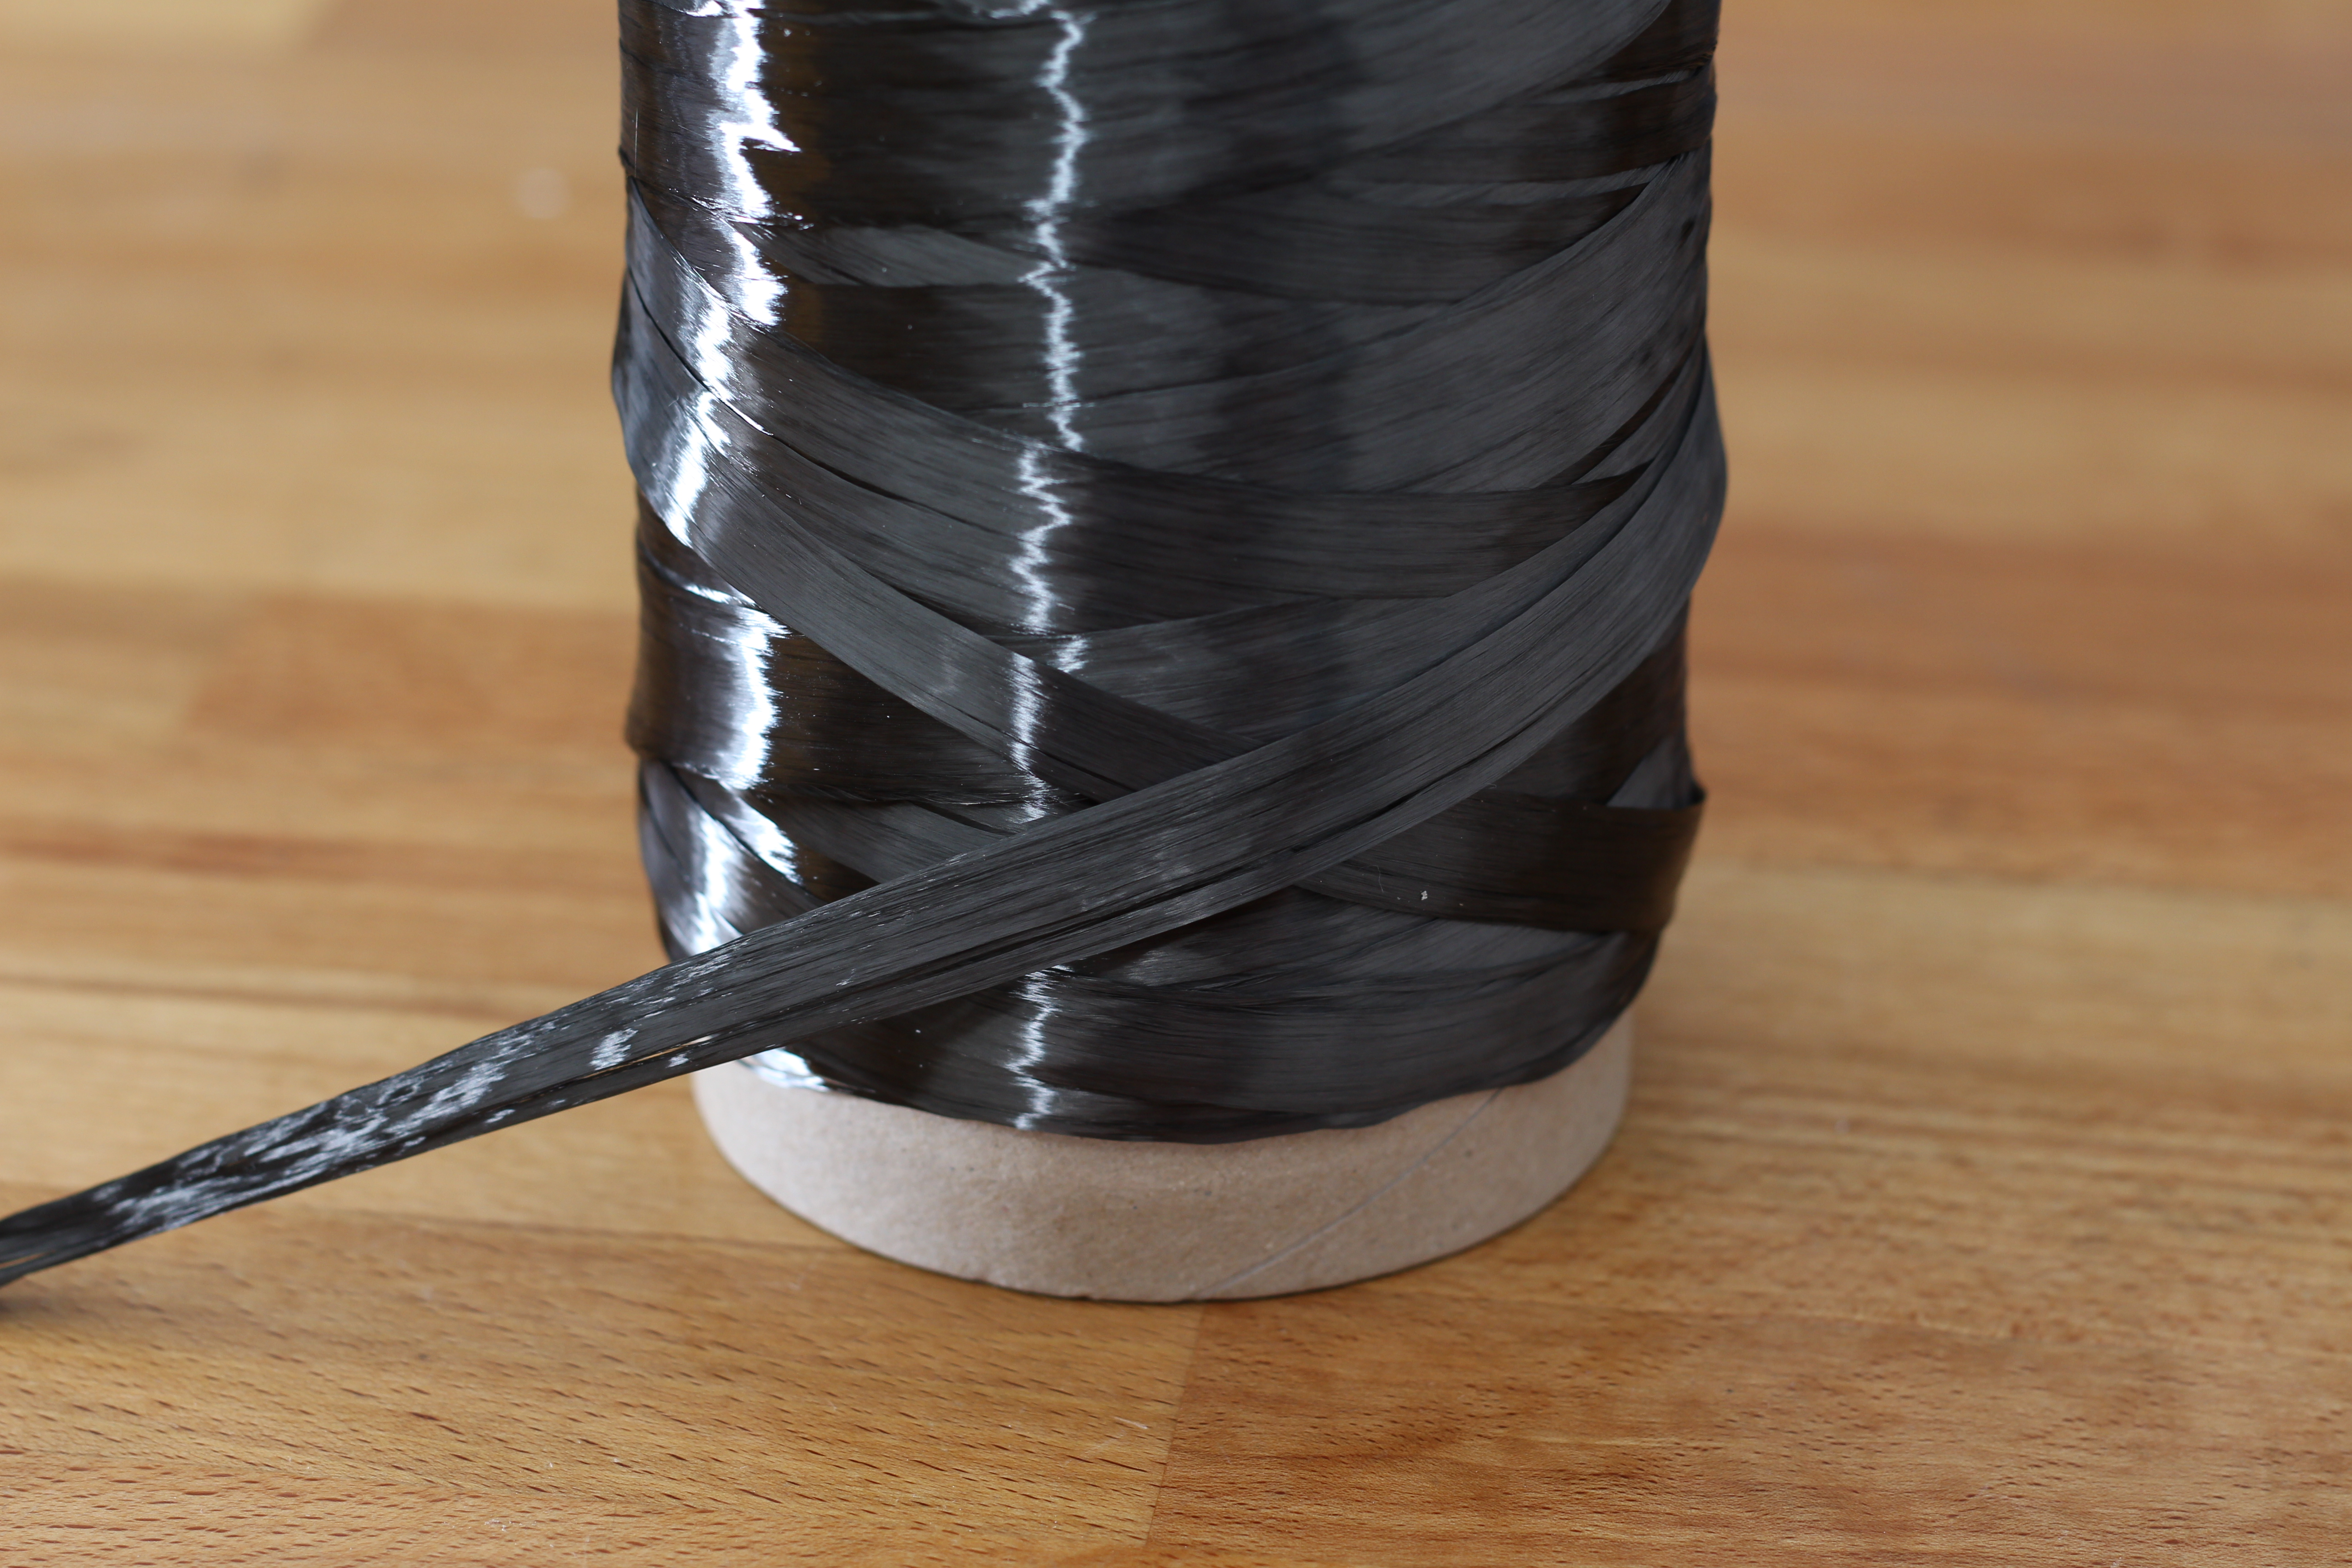
\includegraphics[width=0.8\textwidth]{bilder/IMG_2629.JPG}
%	\caption{Kohlefaserroving} 
%	\label{fig:roving}
%\end{figure}

%Quelle R&G_Handbuch.pdf
%Quelle: http://www.r-g.de/wiki/Was_sind_Faserverbundwerkstoffe%3F

\section{Mathematik zur Beschreibung des Wickelvorgangs}
Um die gewünschten Wickelmuster zu erzeugen ist es wichtig, dieses zuerst mathematisch zu beschreiben. Dies geht am besten im Zylinderkoordinatensystem, wobei die Länge $r$ konstant bleibt und der Winkel $\varphi$ ständig inkrementiert wird, so lange sich der Wickelkörper dreht und damit den Roving aufwickelt. Der Schlitten verfährt dabei in z-Richtung. Dazu ist es nötig die Steigung $s(z)$ der Windung als Weg pro Umdrehung zu definieren. Es gibt für eine komplette Windung, also von $z = 0$ bis $z = z_{max}$ mehrere Zustände des Wickelns.
\begin{itemize}
	\item Anfangsstück: Bereich von $z = 0$ bis $z = z_{start}$
	\item Mitte: Bereich von $z = z_{start}$ bis $z = z_{end}$
	\item Endstück: Bereich von $z = z_{end}$ bis $z = z_{max}$
\end{itemize}
In den drei Abschnitten muss jeweils auf die Steigung eingegangen werden, diese ist nur in der Mitte konstant und lässt sich auch nur hier aus dem vorgegeben Wickelwinkel bestimmen, an den übrigen beiden Stücken ist die Steigung von $z$ abhängig. Das kommt daher, dass eine Windung bei $z = 0$ und $s = 0$ anfängt, da die Steigung beim Umkehren kurzzeitig Null wird und das Umkehren immer bei $z = 0$ und $z = z_{max}$ geschieht. Der Wickelvorgang selbst ist im Zylinderkoordinatensystem durch einen linear steigenden Winkel $\varphi$ und ein abschnittsweise definiertes $s(z)$ zu berechnen. Für den Wickelgang \enquote{vorwärts} ist $s = s(z)$ und rückwärts ist $s = -s(z)$. $s(z)$ muss unbedingt auf dem gesamten Bereich $z \in [0; z_{max}]$ stetig sein, da die Steigung beim Wickeln nicht springen kann, dazu müsste der Roving reißen oder umgesetzt werden, was schlicht physikalisch nicht geht.\\
Komplizierter wird es nun, wenn die Längen von Anfangs- und Endstück nicht gleich sind, da dann die Steigung am Anfang einer anderen Abhängigkeit folgt, als am Ende, um die Stetigkeit von $s$ garantieren zu können. Im einfachsten Falle (Abhängigkeit rein linear) ist $s(z)$ eine lineare Funktion, die die sich aus den Punkten $s(z = 0)$, $s(z = z_{start}$ und $z = z_{max}$ berechnen lässt.\\
\begin{equation}\label{steigungHin}
	s(z)=
	\begin{cases}
		\frac{z}{z_{start}} \cdot s_{soll} & \text{für } z \leq z_{start}\\
		s_{soll} & \text{für } z_{start} \leq z \leq z_{end}\\
		\left( 1 - \frac{z}{z_{max}}\right) \cdot s_{soll} & \text{für } z \leq z_{max}
	\end{cases}	
\end{equation}\\
Damit ist jetzt die Steigung für alle möglichen Fälle definiert, so lange sie sich nur linear verändern darf. Für eine anderweitige Abhängigkeit, Beispielsweise eine exponentielle zu- und Abnahme der Steigung ist die obrige Funktion entsprechend anzupassen. Für die ersten Tests wird darauf jedoch verzichtet und eine rein linaere Funktion gewählt.\\
Eine weitere Schwierigkeit besteht darin, den Roving nach jedem Durchgang zielgenau und mit einem definierten Versatz zum vorherigen Durchgang auf das Rohr aufzubringen. Hierfür ist es wichtig die genaue Breite des Rovings und die gewünschte Mindestüberlappung einzelner Windungen zu kennen. Die Position der Spindeln muss natürlich auch weiterhin exakt sein, es dürfen sich vor allem keine Fehler über die Wickelgänge aufaddieren. Insbesondere die Enden an denen umgekehrt wird und entsprechend beschleunigt bzw. abgebremst werden muss, können dabei zu Problemen führen.\\
Dafür wird jetzt die Windung vom Zylinder- in das kartesische Koordinatensystem umgerechnet, eine Windung setzt sich also aus einem Sinus- und einem Cosinusterm zusammen.\\
\begin{eqnarray}\label{zylinder2kartesischHin}
	x(\varphi) = \sin(\varphi + \varphi_0)\\
	y(\varphi) = \cos(\varphi + \varphi_0)
\end{eqnarray}\\
Der Winkel $\varphi$ wird hierbei ausschließlich inkrementiert und pro Umdrehung wird $\varphi_0$ so erhöht, dass die Rovinglagen sich um einen vorher definierten Wert überlappen. Wichtig hierbei ist, dass $\varphi_0$ nur in ganzzahligen Teilen von \SI{360}{\degree} ansteigt, damit es keine subharmonischen Wellen auf dem Rohr gibt und so überall gleichviel Roving pro Fläche aufgewickelt ist, wenn eine komplette Lage (das sind dann $\frac{360}{\varphi_{0,min}}$ Wickelgänge) fertig ist.\\
Erst nachdem eine komplette Lage voll ist, das heißt, $\varphi_0$ hat \SI{360}{\degree} erreicht, wird $\varphi_0 = 0$ gesetzt und das Rohr ist entweder fertig, sofern die Lagenanzahl auf $1$ steht, oder ein neuer Lagenzyklus beginnt.\\
Um diese Berechnungen zu simulieren, wurde ein Programm in Matlab geschrieben und in 3D geplottet. Wichtig ist hierbei, dass die Formeln \eqref{zylinder2kartesischHin} hier nur für den Wickelvorgang von $z = 0$ ausgehend in positive Richtung angegeben sind. Um von $z = z_{max}$ wieder zurückzukommen, ist es nötig, die Formeln folgendermaßen umzuschreiben:\\
\begin{eqnarray}\label{zylinder2kartesischRueck}
	x(\varphi) = \sin(-(\varphi + \varphi_0))\\
	y(\varphi) = \cos(-(\varphi + \varphi_0))
\end{eqnarray}\\
Die Umschaltung zwischen den beiden Formelsätzen geschieht immer genau am Anfang bzw. Ende eines Wickelvorgangs. Dies kann nicht mehr in einer Funktion untergebracht werden, da dies eine nicht-eindeutige Abbildung ergeben würde, die keine Funktion mehr ist. Deswegen musste die Windung auch im Matlab auf zwei Funktionen in einem Plot aufgesplittet werden. \\
Auch für die Code-Erzeugung spielt dies eine wichtige Rolle. Damit sich die Lagen Vorwärts und Rückwärts maximal überlappen, müssen sie jeweils um \SI{180}{\degree} zueinander verschoben sein. Das heißt, dass beim Wickeln der Endstücke jeweils in Summe eine halbe Umdrehung mehr gewickelt werden muss, als eigendlich durch die Formeln gegeben. Dadurch erweitert sich die Formel \eqref{steigungHin} um je einen Term im ersten und im dritten Abschnitt.\\
In der G-Code-Erzeugungssoftware musste daher darauf geachtet werden, dass der Roving von jeder Wicklung zur nächstgelegenen eine Mindestüberlappung einhält und gleichzeitig die Anzahl der Windungen pro Lage ein Teiler von \SI{360}{\degree} bleibt. Es musste der Kompromiss eingegangen werden, dass das Programm im Zweifel eine leicht zu hohe Überlappung wählt, um die Teilerbedingung unbedingt einzuhalten.\\
Es ist jedoch denkbar, diese Bedingung vom Benutzer abwählbar zu machen, wohlwissend, dass das Rohr dann nicht mehr komplett symmetrisch werden kann, weil die Wicklungen nicht mehr genau \SI{360}{\degree} ergeben und sich an einer Stelle eine minimale Verdickung bildet.\\
Der nächste Schritt für den Wickelprozess ist die Berechnung der Winkel in Relation zu Steigung $s$ und dem zurückzulegenden Weg $z$, wobei besonderes Augenmerk auf die veränderliche Steigung an Anfang und Ende einer jeden Windung und den Winkelverschub $\varphi_0$ gelegt werden muss. Zuerst werden die allgemeinen Gleichungen für die Winkelberechnung dargelegt.\\
Mit der Steigung in $\frac{\text{mm}}{\text{Umdrehung}}$ angegeben ergibt sich folgender Zusammenhang:\\
\begin{equation}\label{SteigungMalWinkel}
	z = s_{soll} \cdot \varphi \quad \iff \quad \varphi = \frac{z}{s_{soll}}
\end{equation}\\
So lange die Steigung $s = s_{soll}$ konstant ist, lässt sich \eqref{steigungHin} so umstellen, dass der Winkel $\varphi$ herauskommt und $z$ sowie $s_{soll}$ angegeben werden müssen. Also genau, wie man das für die Programmierung haben will. Hierbei ergeben sich allerdings keine Verläufe sondern feste Winkelwerte für die zurückzulegenden Strecken.
\begin{equation}\label{GesamtwegeHinRueck}
	\varphi =
	\begin{cases}
		\varphi_0 + \SI{90}{\degree} + \frac{z_{start}}{s_{soll}} & \text{Weg von 0 bis $z_{start}$}\\ 
		\frac{z_{end} - z_{start}}{s_{soll}} & \text{Weg von $z_{start}$ bis $z_{end}$}\\
		\SI{90}{\degree} + \frac{z_{max} - z_{end}}{s_{soll}} & \text{Weg von $z_{end}$ bis $z_{max}$}
	\end{cases}	
\end{equation}\\
Da hier ein linearer Anstieg der Steigung verwendet werden soll, werden die Strecken \enquote{START} und \enquote{ENDE} jeweils in $n$ Punkte zerlegt und innerhalb dieser sei die Steigung jeweils konstant. Weil G-Code sowieso nur endliche Genauigkeit hat, muss an irgend einem Punkt an den exakten Wert angenähert werden, was hier geschieht. Die beiden \SI{90}{\degree} extra kommen daher, dass am Ende eines hin-Wickelganges mit \SI{180}{\degree} Phasenversatz weitergewickelt werden muss und das $\varphi_0$ ist, wie schon erwähnt, für den Phasenversatz zwischen den einzelnen Wickelgängen.\\
Die jeweiligen $n$ Punkte werden mit der Formel \eqref{steigungHin} auf jeweils $\frac{\varphi}{n}$ Drehwinkel berechnet und direkt als G-Code ausgegeben.


% needed in second column of first page if using \IEEEpubid
%\IEEEpubidadjcol

\section{Mechanischer Aufbau}
\subsection{Konzept}
Der Grundaufbau der Wickelmaschine gleicht dem einer Drehbank. Es gibt eine Drehachse die den Wickelkörper rotiert, sowie einen Arm der auf einer Achse längs dem Wickelkörper bewegt wird. Dieser Arm führt den Roving und sorgt für eine exakte Platzierung, weshalb der Arm zusätzlich senkrecht zur Wickelachse bewegbar und rotierbar ist. Auf diese Weiße lässt sich der Abstand zwischen Wickelkörper und Arm variieren sowie die Orientierung an den aktuellen Wickelwinkel anpassen. Zur Ansteuerung der Achsen kommen Schrittmotoren zum Einsatz, da diese zum einen vergleichsweise einfach und kostengünstig ansteuerbar sind und zum andern fertige Module mit Steppertreibern verfügbar sind. Über den oben beschriebenen drehbaren Arm wird der Roving zum Wickelkörper geführt, wobei dieser zuvor mit Epoxydharz getränkt werden muss, da dies je nach Gewebedicke nach dem Wickeln nur schlecht möglich ist. Außerdem ist durch die vorgesehene automatische Tränk- und Abstreifvorrichtung eine gleichmäßige Harzmenge garantiert. Durch eine variable Positionierung des Reitstocks sind Wickelkörper in fast beliebigen Längen und Durchmessern, bis zu \SI{1200}{\milli\metre} Länge und unter \SI{250}{\milli\metre} Durchmesser, möglich.


\section{Mechanik}
Der mechanische Aufbau der Wickelmaschine wurde, soweit nötig, als 3D-Modell erstellt. Manche Details wie Schrauben wurden dabei an irrelevanten Stellen weggelassen. Das Augenmerk liegt insbesondere auf den Teilen die in der Fräse selbst herzustellen sind, wie z.B. die Motorhalterungen, der Reitstock und die Verbindungen zu Teilen wie den Schrittmoten. Außerdem lässt sich in dem Maschinenmodell überprüfen, dass die Verbindungen und Lage der verschiedenen Teile zueinander stimmt. Im Folgenden sollen die einzelnen Teile der Wickelmaschine näher betrachtet und erklärt werden.

\subsection{Grundplatte}
Die Grundplatte dient als Aufnahme für die weiteren Teile wie Spindel, Reitstock, Linearführungen, usw. Aus Kosten- und Gewichtsgründen wird diese aus Multiplexplatte hergestellt, weil die Festigkeit für die zu erwartende geringe mechanische Belastung ausreichend ist. Auf dieser müssen Spindelhalter, Reitstock und die lange Linearführung montiert werden. Der Reitstock ist zusätzlich verschiebbar um die Maschine auf verschieden lange Wickelkörper anpassen zu können.

\subsection{Spindel}
Die Spindel nimmt eine Seite des Wickelkörpers auf und treibt diesen mithilfe eines Schrittmotors an. Die Aufnahme für den Wickelkörper ist kegelförmig um unterschiedlich große Rohrdurchmesser von innen Spannen zu können. Die Kraftübertragung geschieht über Reibung wie bei einer Drehbank, in der Material zwischen Spitzen gespannt ist. Für spezielle Wickelkörper ist der Kegel zusätzlich noch austauschbar. In der Achsenbeschreibung hat diese Achse den Buchstaben C, also parallel zur linearen Achse Z gelegen.

%\begin{figure}[H]
%	\centering
%	\includegraphics[width=0.8\textwidth]{NX_Screenshots/spindel.png}
%	\caption{angetriebene Spindel inkl. Halterung und Aufnahmekegel} 
%	\label{fig:spindel}
%\end{figure}

\subsection{Reitstock}
Am Reitstock wird der Wickelkörper leicht drehbar gegengelagert. Um unterschiedlich lange Wickelkörper verwenden zu können ist dieser in Z-Richtung stufenlos verschiebbar. Der Aufbau ist ähnlich dem der Spindel mit Ausnahme des fehlenden Antriebs. Zusätzlich ist eine Feder vorgesehen die den Kegel auf den Wickelkörper drückt. Dies ermöglicht ein einfacheres Wechseln des Wickelkörpers, ohne den Reitstock selbst verschieben zu müssen.


\subsection{Wickelwagen}
Der Wickelwagen lagert auf einer langen Linearführung und führt den eigentlichen Wickelvorgang aus. Da darauf später nicht wenig Gewicht lagert, muss er robust ausgeführt und gegen Verkippen gesichert sein. Wir haben uns entschieden, eine Linearführung mit Kugelumlauflagerung im Wagen zu kaufen und nicht auf sonst im Hobbybereich anzutreffende unterstützte Wellen oder Schubladenschienen zurückzugreifen.\\
Der Wagen führt demnach die Bewegung in der Achse Z aus und trägt eine weitere, kleine Linearführung, die dann die Bewegung in X-Richtung ermöglicht. Damit entspricht der Wagen dem Planschlitten einer Drehbank. Die folgenden Abbildungen zeigen die verwendeten Linearführungen.

%\begin{figure}[H]
%	\centering
%	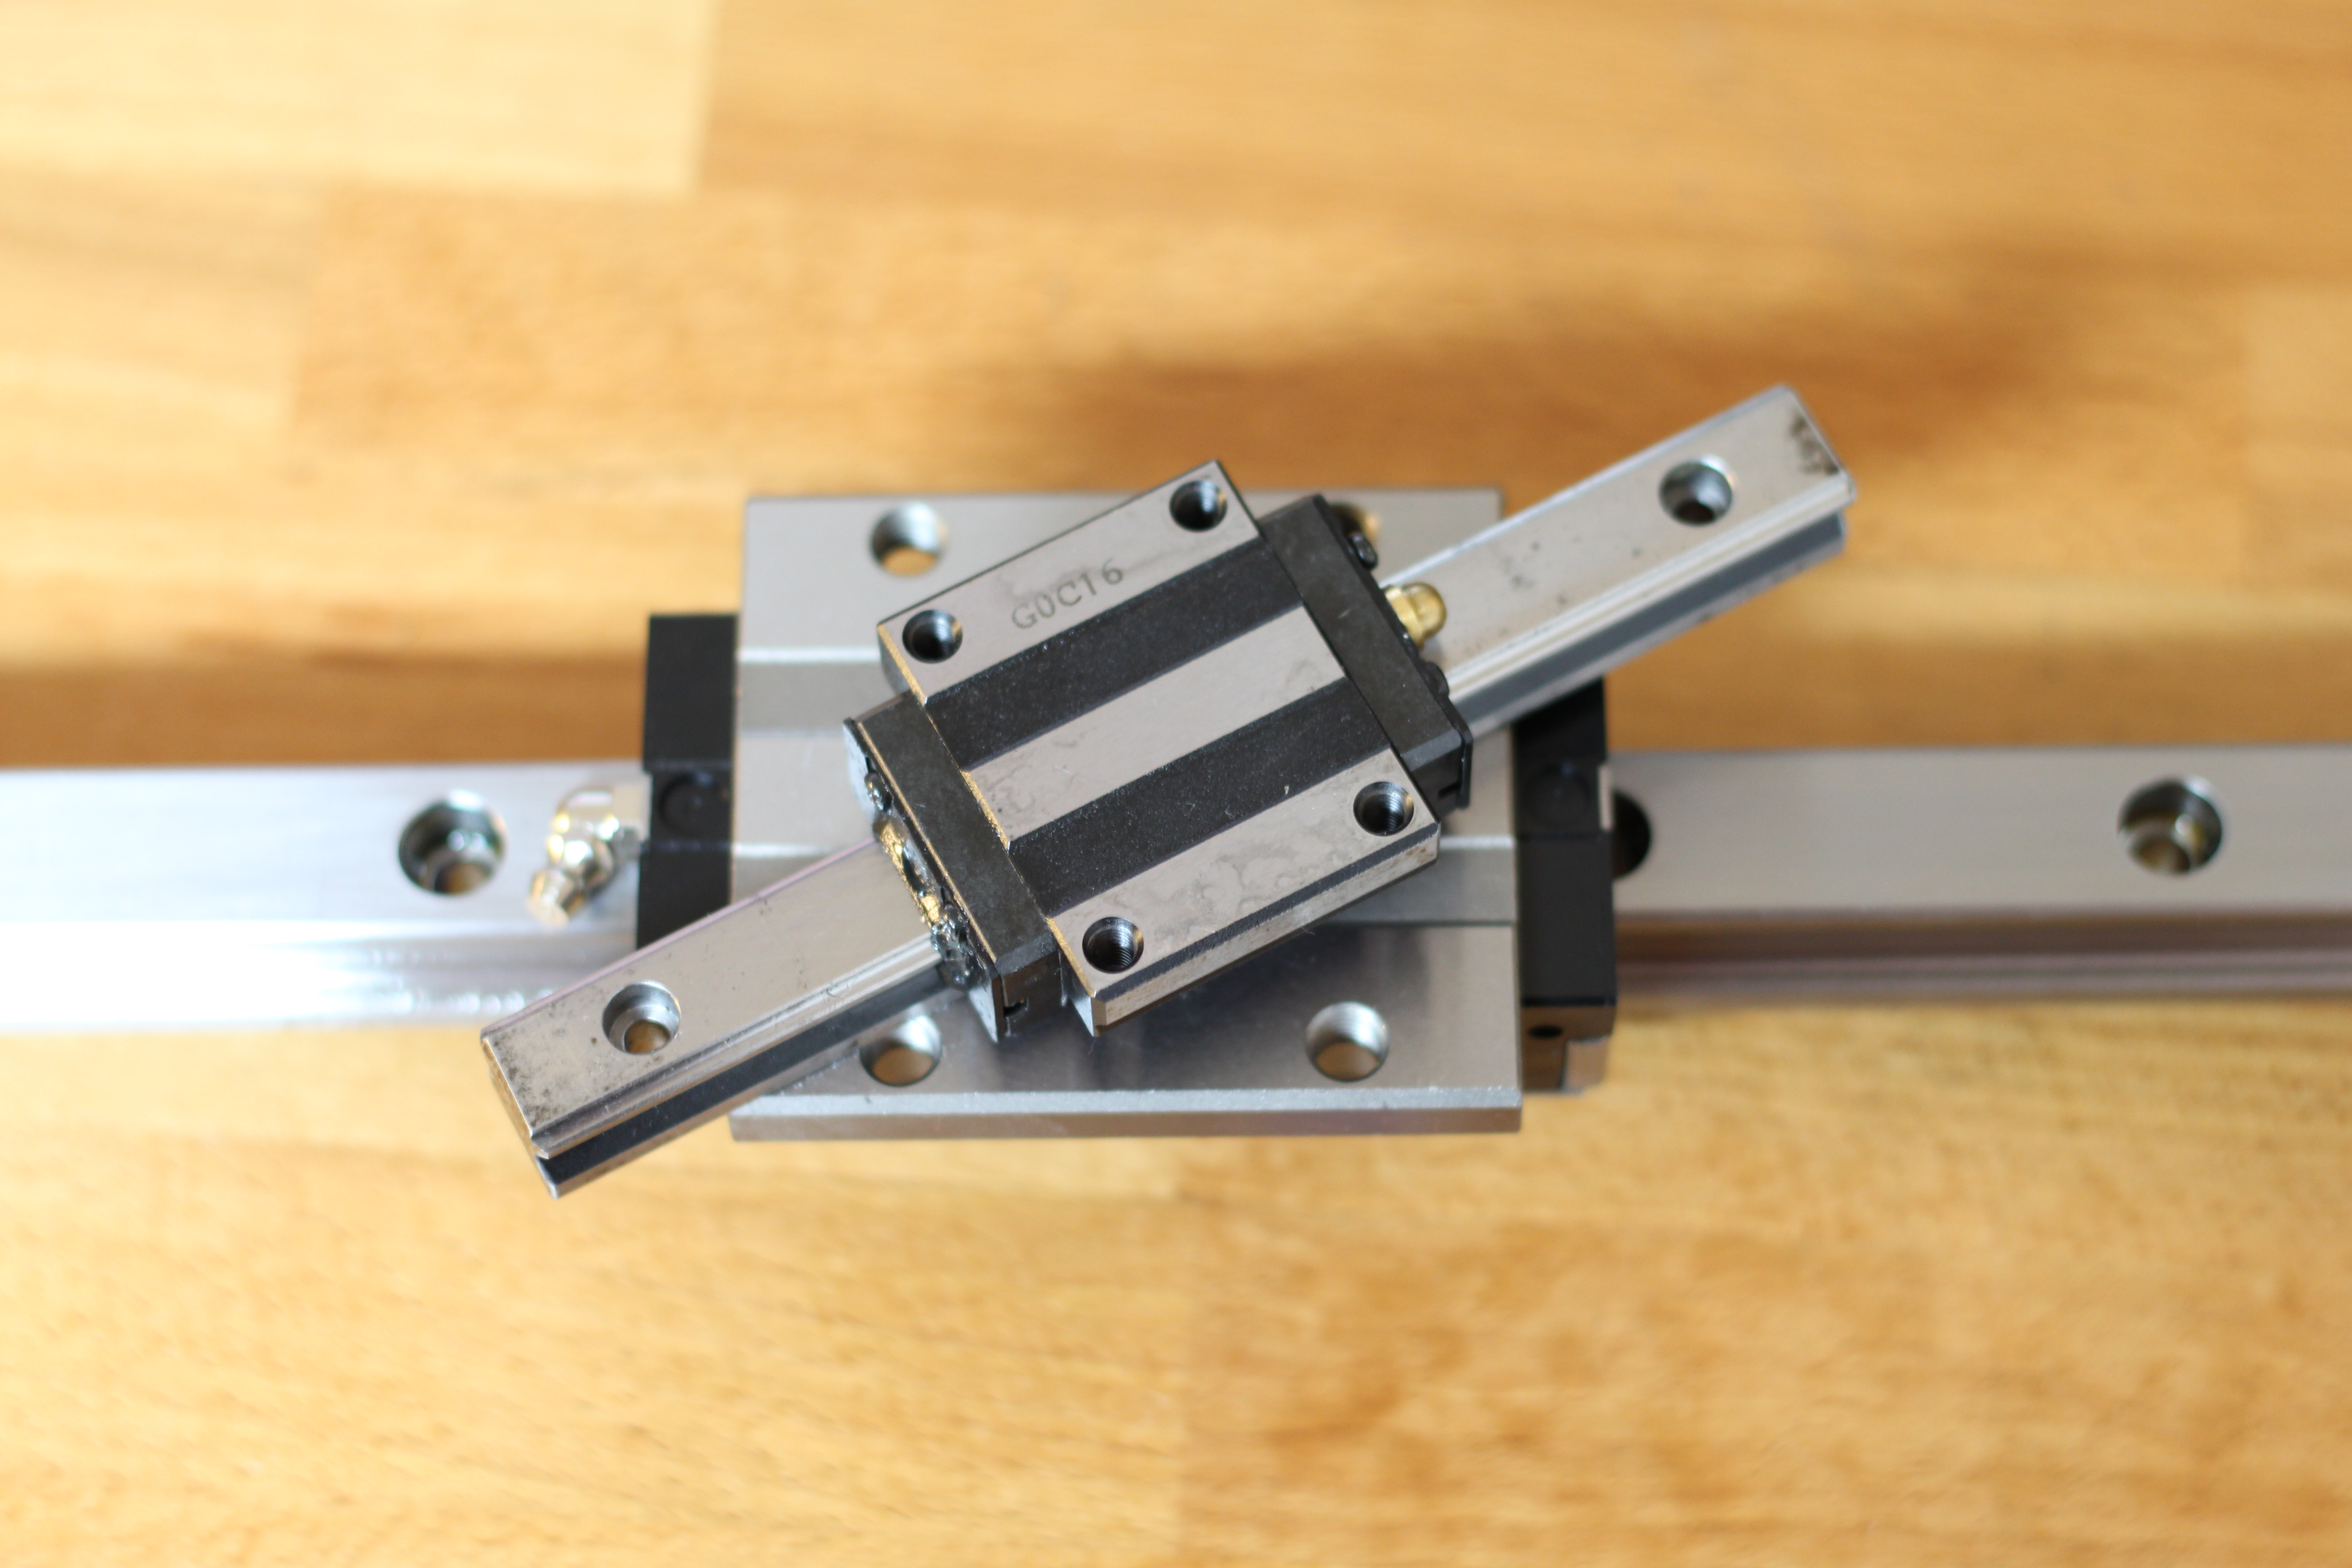
\includegraphics[width=0.8\textwidth]{bilder/IMG_2616.JPG}
%	\caption{Linearführungen im demontierten Zustand} 
%	\label{fig:wagen}
%\end{figure}
%
%\begin{figure}[H]
%	\centering
%	\includegraphics[width=0.8\textwidth]{NX_Screenshots/wagen.png}
%	\caption{Wagen der Linearführung in NX} 
%	\label{fig:wagen_foto}
%\end{figure}
%
%
%\subsection{Dreharm}
%\begin{figure}
%	\centering
%	\includegraphics[width=0.8\textwidth]{NX_Screenshots/arm_vorne.png}
%	\caption{Dreharm mit Rovingführung} 
%	\label{fig:dreharm}
%\end{figure}
In Abbildung \ref{fig:dreharm} sieht man die Adapterplatte, die auf dem Wickelwagen (unten in der Mitte) befestigt wird. Das senkrechte Blechstück trägt dann einen weiteren Schrittmotor und den Rovingdurchlass mit der Dreheinheit. Diese sorgt dafür, dass auch bei komplexeren Wickelgeometrien, wie beispielsweise Flaschen oder unterschiedlich dicken Gegenständen, der Roving stets korrekt positioniert wird. Auf einer CNC-Maschine wäre dies die zur X-Achse parallele Drehachse, die dann mit dem Buchstaben A bezeichnet wird. Da der Roving zum Zeitpunkt des Wickelns schon mit Harz getränkt ist, müssen alle Teile, die mit dem Roving in Berührung kommen, aus Teflon hergestellt werden. Hier trifft das auf die kleine Umlenkrolle vorne am Drehaufsatz zu, diese wird durch zwei Schrauben gehalten und ist so leicht ausbaubar oder sogar austauschbar.\\
Der Antrieb der X-Achse ist hier ausgeblendet, um die Drehvorrichtung der Achse A besser zeigen zu können.


\subsection{Tränkeinheit}
Bevor das Roving auf den Wickelkörper aufgebracht werden kann muss es zuerst mit Harz getränkt werden. Zu diesem Zweck ist ein Gefäß vorgesehen, das auf dem Wagen in Z und X Richtung mitfährt und mit einer ausreichenden Menge an Harz gefüllt ist. Dabei wurde darauf geachtet, dass möglichst wenig Harz in dem Behälter verbleibt und verschwendet wird. Im wesentlichen läuft das Roving in der Tränkeinheit über zwei Umlenkungen und einen Abstreifer an dem das überschüssige Harz entfernt und dem Behälter wieder zugeführt wird. Anschließend läuft das Roving nur noch durch den Dreharm und dessen Umlenkrolle aus Teflon um die Anzahl der zu reinigenden Teile gering zu halten.
%\begin{figure}[H]
%	\centering
%	\includegraphics[angle=270, width=1\textwidth]{bilder/skizze.jpg}
%	\caption{Skizze der Tränkeinrichtung} 
%	\label{fig:123}
%\end{figure}



\section{Software}
Die verwendete Software besteht aus zwei Teilen die im folgenden näher beschrieben werden. Zum einen einem Programm zur G-Code Erzeugung, zum anderen einem Interface zur Maschinensteuerung.
\subsection{G-Code Erzeugung}
\label{software}
Die Steuerung der Wickelmaschine erfolgt über normale G-Code Kommandos wie sie auch bei vielen anderen CNC-Maschinen verwendet werden. Für Fräs- und Drehmaschinen gibt es zur Erzeugung von G-Code anhand eine CAD Modells bereits viele Programme, für Wickelmaschinen leider nur sehr wenige und noch dazu sehr teure. Deshalb wurde auf Basis des unter \ref{mathematik} beschriebenen mathematischen Modells eine PC-Software in C++ entwickelt die  anhand der eingestellten Parameter passenden G-Code erzeugt. In Abbildung \ref{fig:g-code} ist das graphische Userinterface zu sehen. 
%\begin{figure}[H]
%	\centering
%	\includegraphics[width=1\textwidth]{bilder/carbowickler_software.png}
%	\caption{Programm zur G-Code Erzeugung} 
%	\label{fig:g-code}
%\end{figure}


\subsection{grbl Interface}
Die verwendete Steuerung basiert auf grbl\cite{grbl}, welches bis zu vier Schrittmotoren anhand von G-Code ansteuert. Zum Übertragen des G-Codes an die Steuerung existieren bereits mehrere fertige Programme die eingesetzt werden können, weshalb es nicht nötig ist hierfür ein Neues zu entwickeln. Stattdessen ging es primäre darum G-Code zu erzeugen der zu dem gewünschten Wickelmuster führt, siehe hierzu \ref{software}. Die Hardware der Steuerung ist in \ref{fig:grbl_board} zu sehen.
%\begin{figure}[H]
%	\centering
%	\includegraphics[width=1\textwidth]{bilder/IMG_2662.JPG}
%	\caption{grbl-board mit stepsticks} 
%	\label{fig:grbl_board}
%\end{figure}




% An example of a floating figure using the graphicx package.
% Note that \label must occur AFTER (or within) \caption.
% For figures, \caption should occur after the \includegraphics.
% Note that IEEEtran v1.7 and later has special internal code that
% is designed to preserve the operation of \label within \caption
% even when the captionsoff option is in effect. However, because
% of issues like this, it may be the safest practice to put all your
% \label just after \caption rather than within \caption{}.
%
% Reminder: the "draftcls" or "draftclsnofoot", not "draft", class
% option should be used if it is desired that the figures are to be
% displayed while in draft mode.
%
%\begin{figure}[!t]
%\centering
%\includegraphics[width=2.5in]{myfigure}
% where an .eps filename suffix will be assumed under latex, 
% and a .pdf suffix will be assumed for pdflatex; or what has been declared
% via \DeclareGraphicsExtensions.
%\caption{Simulation results for the network.}
%\label{fig_sim}
%\end{figure}

% Note that the IEEE typically puts floats only at the top, even when this
% results in a large percentage of a column being occupied by floats.


% An example of a double column floating figure using two subfigures.
% (The subfig.sty package must be loaded for this to work.)
% The subfigure \label commands are set within each subfloat command,
% and the \label for the overall figure must come after \caption.
% \hfil is used as a separator to get equal spacing.
% Watch out that the combined width of all the subfigures on a 
% line do not exceed the text width or a line break will occur.
%
%\begin{figure*}[!t]
%\centering
%\subfloat[Case I]{\includegraphics[width=2.5in]{box}%
%\label{fig_first_case}}
%\hfil
%\subfloat[Case II]{\includegraphics[width=2.5in]{box}%
%\label{fig_second_case}}
%\caption{Simulation results for the network.}
%\label{fig_sim}
%\end{figure*}
%
% Note that often IEEE papers with subfigures do not employ subfigure
% captions (using the optional argument to \subfloat[]), but instead will
% reference/describe all of them (a), (b), etc., within the main caption.
% Be aware that for subfig.sty to generate the (a), (b), etc., subfigure
% labels, the optional argument to \subfloat must be present. If a
% subcaption is not desired, just leave its contents blank,
% e.g., \subfloat[].


% An example of a floating table. Note that, for IEEE style tables, the
% \caption command should come BEFORE the table and, given that table
% captions serve much like titles, are usually capitalized except for words
% such as a, an, and, as, at, but, by, for, in, nor, of, on, or, the, to
% and up, which are usually not capitalized unless they are the first or
% last word of the caption. Table text will default to \footnotesize as
% the IEEE normally uses this smaller font for tables.
% The \label must come after \caption as always.
%
%\begin{table}[!t]
%% increase table row spacing, adjust to taste
%\renewcommand{\arraystretch}{1.3}
% if using array.sty, it might be a good idea to tweak the value of
% \extrarowheight as needed to properly center the text within the cells
%\caption{An Example of a Table}
%\label{table_example}
%\centering
%% Some packages, such as MDW tools, offer better commands for making tables
%% than the plain LaTeX2e tabular which is used here.
%\begin{tabular}{|c||c|}
%\hline
%One & Two\\
%\hline
%Three & Four\\
%\hline
%\end{tabular}
%\end{table}


% Note that the IEEE does not put floats in the very first column
% - or typically anywhere on the first page for that matter. Also,
% in-text middle ("here") positioning is typically not used, but it
% is allowed and encouraged for Computer Society conferences (but
% not Computer Society journals). Most IEEE journals/conferences use
% top floats exclusively. 
% Note that, LaTeX2e, unlike IEEE journals/conferences, places
% footnotes above bottom floats. This can be corrected via the
% \fnbelowfloat command of the stfloats package.




\section{Conclusion}
The conclusion goes here.





% if have a single appendix:
%\appendix[Proof of the Zonklar Equations]
% or
%\appendix  % for no appendix heading
% do not use \section anymore after \appendix, only \section*
% is possibly needed

% use appendices with more than one appendix
% then use \section to start each appendix
% you must declare a \section before using any
% \subsection or using \label (\appendices by itself
% starts a section numbered zero.)
%


\appendices
\section{Proof of the First Zonklar Equation}
Appendix one text goes here.

% you can choose not to have a title for an appendix
% if you want by leaving the argument blank
\section{}
Appendix two text goes here.


% use section* for acknowledgment
\section*{Acknowledgment}


The authors would like to thank...


% Can use something like this to put references on a page
% by themselves when using endfloat and the captionsoff option.
\ifCLASSOPTIONcaptionsoff
  \newpage
\fi



% trigger a \newpage just before the given reference
% number - used to balance the columns on the last page
% adjust value as needed - may need to be readjusted if
% the document is modified later
%\IEEEtriggeratref{8}
% The "triggered" command can be changed if desired:
%\IEEEtriggercmd{\enlargethispage{-5in}}

% references section

% can use a bibliography generated by BibTeX as a .bbl file
% BibTeX documentation can be easily obtained at:
% http://mirror.ctan.org/biblio/bibtex/contrib/doc/
% The IEEEtran BibTeX style support page is at:
% http://www.michaelshell.org/tex/ieeetran/bibtex/
%\bibliographystyle{IEEEtran}
% argument is your BibTeX string definitions and bibliography database(s)
%\bibliography{IEEEabrv,../bib/paper}
%
% <OR> manually copy in the resultant .bbl file
% set second argument of \begin to the number of references
% (used to reserve space for the reference number labels box)
\begin{thebibliography}{1}

\bibitem{r_g_handbuch}
R\&G Handbuch Faserverbundwerkstoffe
%@ONLINE{grbl,
%  author		= {Simen Svale Skogsrud, Sungeun K. Jeon},
%  title			= {GRBL},
%  month			= jan,
%  year			= {2016},
%  url			= {https://github.com/grbl/grbl}
%}
%
%@ONLINE{r_g_wiki,
%  author		= {R\&G Faserverbundwerkstoffe GmbH},
%  title			= {R\&G Wiki},
%  month			= jan,
%  year			= {2016},
%  url			= {http://www.r-g.de/wiki/Was_sind_Faserverbundwerkstoffe%3F}
%}
%@manual{r_g_handbuch,
%  organization	= {R\&G Faserverbundwerkstoffe GmbH},
%  address       = "D-71111 Waldenbuch",
%  title			= {R\&G Handbuch Faserverbundwerkstoffe},
%  month			= jun,
%  year			= {2009},
%  url			= {http://www.r-g.de/w/images/6/69/R%26G_Handbuch.pdf}
%}

%\bibitem{IEEEhowto:kopka}
%H.~Kopka and P.~W. Daly, \emph{A Guide to \LaTeX}, 3rd~ed.\hskip 1em plus
%  0.5em minus 0.4em\relax Harlow, England: Addison-Wesley, 1999.

\end{thebibliography}

% biography section
% 
% If you have an EPS/PDF photo (graphicx package needed) extra braces are
% needed around the contents of the optional argument to biography to prevent
% the LaTeX parser from getting confused when it sees the complicated
% \includegraphics command within an optional argument. (You could create
% your own custom macro containing the \includegraphics command to make things
% simpler here.)
%\begin{IEEEbiography}[{\includegraphics[width=1in,height=1.25in,clip,keepaspectratio]{mshell}}]{Michael Shell}
% or if you just want to reserve a space for a photo:

%\begin{IEEEbiography}{Michael Shell}
%Biography text here.
%\end{IEEEbiography}
%
%% if you will not have a photo at all:
%\begin{IEEEbiographynophoto}{John Doe}
%Biography text here.
%\end{IEEEbiographynophoto}
%
%% insert where needed to balance the two columns on the last page with
%% biographies
%%\newpage
%
%\begin{IEEEbiographynophoto}{Jane Doe}
%Biography text here.
%\end{IEEEbiographynophoto}

% You can push biographies down or up by placing
% a \vfill before or after them. The appropriate
% use of \vfill depends on what kind of text is
% on the last page and whether or not the columns
% are being equalized.

%\vfill

% Can be used to pull up biographies so that the bottom of the last one
% is flush with the other column.
%\enlargethispage{-5in}



% that's all folks
\end{document}


